

\section{Introduction}

\begin{frame}
	\frametitle{Problem Size/Compute Time Correlation}
		\begin{columns}[c] 

			\column{.5\textwidth} % Left column and width
			\begin{figure}
					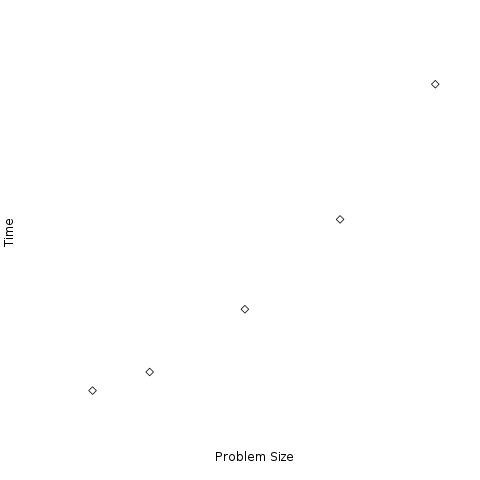
\includegraphics[width=0.85\linewidth]{figures/time/laplace}
			\end{figure}
			\column{.5\textwidth} % Right column and width

			\begin{figure}
			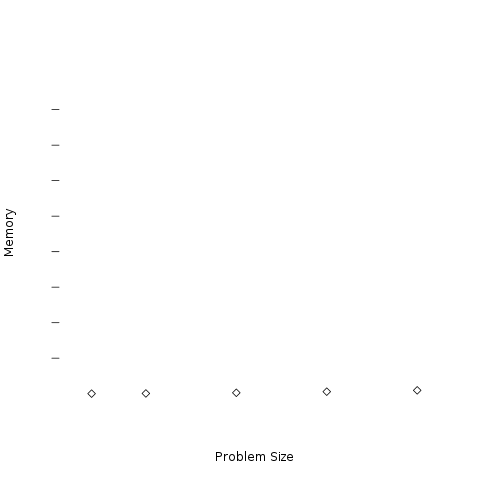
\includegraphics[width=0.85\linewidth]{figures/memory/laplace}
			\end{figure}
		\end{columns}
\end{frame}

\begin{frame}
	\frametitle{Problem Size/Compute Time Correlation}
		\begin{columns}[c] 

			\column{.5\textwidth} % Left column and width
			\begin{figure}
					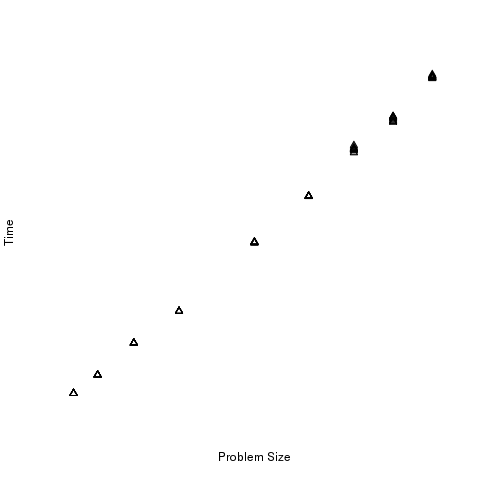
\includegraphics[width=0.85\linewidth]{figures/time/linpack}
			\end{figure}
			\column{.5\textwidth} % Right column and width

			\begin{figure}
			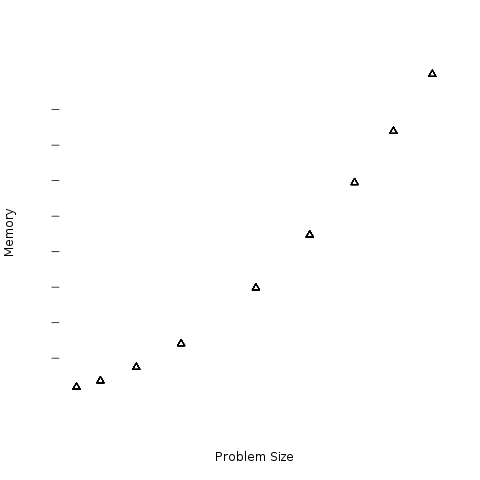
\includegraphics[width=0.85\linewidth]{figures/memory/linpack}
			\end{figure}
		\end{columns}
\end{frame}

\begin{frame}
		\frametitle{Combinations}

\begin{table}
\begin{tabular}{l l}
\toprule
\textbf{Limitation} & \textbf{Solution} \\
\midrule
Compute time only & Parallel Computing \\
Memory only & Distributed Computing \\
Compute time and Memory & Distributed Computing \\
\bottomrule
\end{tabular}
\caption{Method needed given Limitation}
\end{table}
\end{frame}
